\input ../preamble

\begin{document}

{\Huge
  \centerline{\bf TTIC 31230, Fundamentals of Deep Learning}
  \bigskip
  \centerline{David McAllester, Winter 2018}
  \vfill
  \centerline{\bf Gradients as Dual Vectors }
  \vfill
  \centerline{\bf Hessian-Vector Products}
  \vfill
  \centerline{\bf Information Geometry}

\slide{Coordinates}

For a vector space we can make an arbitrary choice of basis vectors $b_1$, $\ldots$, $b_N$
that are linearly independent and span the space.

\vfill
A basis defines coordinates $x[i]$ for each vector $x$.

$$x = x[1]b_1 + \cdots + x[N] b_N$$

\vfill
The basis, and the induced coordinate system, is arbitrary.

\slide{Orthogonality is Coordinate-Relative}

\vfill
In two dimensions the vectors represented by $(1,0)$ and $(0,1)$ need not be orthogonal.

\vfill
$(1,0)$ represents $b_1$ and $(0,1)$ represents $b_2$.

\vfill
We only require that $b_1$ and $b_2$ are independent.

\vfill
Hence inner product is coordinate-relative.


\slidetwo{Inner Products in Taylor Expansions}{are Coordinate-Independent}

$$f(\Phi + \Delta\Phi) \approx f(\Phi) + {\color{red} \left[\nabla_\Phi \;f(\Phi)\right](\Delta \Phi)}$$

\slide{What is a Gradient?}

The gradient $\nabla_\Phi \; f(\Phi)$ is the change in $f$ per change in $\Phi$.

\vfill
More formally, $\nabla_\Phi\; f(\Phi)$ is a linear function from $\Delta \Phi$ to $\Delta f$.

\vfill
$$f(\Phi + \Delta\Phi) \approx f(\Phi) + {\color{red} \left[\nabla_\Phi \;f(\Phi)\right](\Delta \Phi)}$$

\slide{Coordinate-Free Definition of the Gradient}

\begin{eqnarray*}
f(\Phi + \Delta\Phi) \approx f(\Phi) + \left[\nabla_\Phi \;f(\Phi)\right](\Delta \Phi) \\
\\
f(\Phi + \epsilon \Delta\Phi) \approx f(\Phi) + \left[\nabla_\Phi \;f(\Phi)\right](\epsilon \Delta \Phi) \\
\\
\frac{f(\Phi + \epsilon \Delta\Phi) - f(\Phi)}{\epsilon} \approx \left[\nabla_\Phi \;f(\Phi)\right](\Delta \Phi)
\end{eqnarray*}

\vfill

$${\color{red} \left[\nabla_\Phi\; f(\Phi)\right](\Delta \Phi) \;\;\doteq\;\; \lim_{\epsilon \rightarrow 0} \; \frac{f(\Phi + \epsilon \Delta \Phi) - f(\Phi)}{\epsilon}}$$

\vfill
No coordinates required.

\slide{Dual Vectors}

A dual vector is a linear function from vectors to scalars.

\vfill
The gradient is a dual vector.

\slide{Coordinates}

We calculate $$\left[\nabla_\Phi f(\Phi)\right]\Delta \Phi$$  using coordinates.

$$\left[\nabla_\Phi f(\Phi)\right]\Delta \Phi \;\;\;=\;\;\; \sum_i \left[\frac{\partial f}{\partial \Phi[i]}\right] \Delta \Phi[i]$$

\vfill
But this calculation is coordinate-independent.

\vfill
$$\left[\nabla_\Phi\; f(\Phi)\right](\Delta \Phi) \;\;\equiv\;\; \lim_{\epsilon \rightarrow 0} \; \frac{f(\Phi + \epsilon \Delta \Phi) - f(\Phi)}{\epsilon}$$

\slide{Strange Coordinate Systems}

Consider any gradient $\nabla_\Phi f(\Phi)$ at any value of $\Phi$.

\vfill
For any such situation, and {\color{red} any vector $\Delta \Phi$} with $\left[\nabla_\Phi f(\Phi)\right] \Delta \Phi > 0$,
and {\color{red} any learning rate $\eta > 0$},
{\color{red} there exists a coordinate system} in which ${\color{red} \eta \Phi.\mathrm{grad}[c] = \Delta \Phi[c]}$ and hence

\vfill
$${\color{red} \Phi_{t+1} = \Phi_t - \Delta \Phi}$$

\vfill
Note that gradient decent always yields $\left[\nabla_\Phi f(\Phi)\right] \Delta \Phi > 0$.

\slide{Proof}
Define the basis vectors $b_1$, $\ldots$, $b_N$ by

\vfill
$$b_1 \doteq \frac{\Delta \Phi}{\sqrt{\eta[\nabla_\Phi f(\Phi)]\Delta \Phi}} \;\;\;\;\;
{\color{red} \left[\nabla_\Phi f(\Phi)\right]\;b_i = 0} \;\;\mbox{for $i > 1$}$$

In this coordinate system we have
$$\Phi = \Phi[1]b_1 + \ldots + \Phi[N]b_n$$

\vfill
$$\frac{\partial f(\Phi)}{\partial \Phi[1]} = \frac{\sqrt{[\nabla_\Phi f(\Phi)]\Delta \Phi}}{\sqrt{\eta}} \;\;\;\;\;\;
\frac{\partial f(\Phi)}{\partial \Phi[j]} = 0 \;\;\;\mbox{for $j > 0$}$$

\vfill
$$\sum_i \Phi.\mathrm{grad}[i]\Phi[i]b_i = \frac{\sqrt{[\nabla_\Phi f(\Phi)]\Delta \Phi}}{\sqrt{\eta}}\;b_1 = \frac{\Delta \Phi}{\eta}$$

\slide{}
\centerline{\bf Coordinate-Free Versions of SGD}
\vfill
\vfill

\slide{Newton's Method}

We can make a second order approximation to the loss function

\vfill
$$f(\Phi + \Delta \Phi) \approx f(\Phi) + (\nabla_\Phi \;f(\Phi))\Delta \Phi + \frac{1}{2} \Delta \Phi^\top H \Delta \Phi$$

\vfill
where $H$ is the second derivative of $f$, the Hessian, equal to $\nabla_\Phi \nabla_\Phi \;f(\Phi)$.

\vfill
Again, no coordinates are needed --- we can define the operator $\nabla_\Phi$ generally indpendent of coordinates.

\vfill
$$\Delta \Phi_1^\top\;H\; \Delta \Phi_2 = \left(\nabla_\Phi \left((\nabla_\Phi\; f_t(\Phi))\cdot \Delta \Phi_1\right)\right)\cdot \Delta \Phi_2$$

\slide{Newton's Method}

We consider the first order expansion of the gradient.

$$\nabla_\Phi\; f(\Phi)\; |_{\Phi + \Delta \Phi}\approx \left(\nabla _\Phi \;f(\Phi)\; |_{\Phi}\right) + H \Delta \Phi$$

\vfill
We approximate $\Phi^*$ by setting this gradient approximation to zero.

\vfill
\begin{eqnarray*}
  0 & = & \nabla _\Phi\; f(\Phi) + H \Delta \Phi \\
  \\
\Delta \Phi & = & - H^{-1} \;\nabla _\Phi \; f(\Phi)
\end{eqnarray*}

\vfill
This gives Newton's method (without coordinates)

\vfill
{\color{red} $$\Phi \;\minuseq \; H^{-1}\; \nabla_\Phi \;f(\Phi)$$}

\slideplain{Newton Updates}

It seems safer to take smaller steps.  So it is common to use

\vfill
$$\Phi\;\;\minuseq \;\; {\color{red} \eta}\; H^{-1}\;\nabla_\Phi\; f(\Phi)$$

\vfill
for $\eta \in (0,1)$ where $\eta$ is naturally dimensionless.

\vfill
Most second order methods attempt to approximate making updates in the Newton direction.

\slide{The Gradient Covariance Martix}

$$\Sigma \doteq E_t \;(\hat{g}_t - g)(\hat{g}_t - g)^\top$$

\vfill
$$\Phi_{t+1} = \Phi_t - \eta \Sigma^{-1} \nabla_\Phi \mathrm{Loss}(\Phi,x_t,y_y)$$

\vfill
This is related to RMSProp.

\slide{Information Geometry and the Natural Gradient}

We consider the case where loss is determined by a probability distribution.  For example $- \log P(y)$.

\vfill
The set of all distributions $P$ forms a manifold.

\vfill
For a given point (distribution) $P$ we can consider the ball

\vfill
$$B_\epsilon(P) = \{Q \;|\; KL(P,Q) \leq \epsilon\}$$

$$\Delta P = \argmin_{\Delta P \in B_\epsilon(P)} f(P + \Delta P)$$

\slide{Distance Functions Define a Point-Wise Inner Product}

\vfill
For any smooth (doubly differentiable) function $d(x,y)$ with $d(x,y) \geq 0$ and $d(x,x) = 0$
we must have

\vfill
$$\nabla_{\Delta x} \;d(x,x+ \Delta x)|_{\Delta x = 0} = 0$$
\begin{eqnarray*}
d(x,x + \Delta x) \approx \Delta x^\top H \Delta x \\
\\
H \doteq \nabla_{\Delta x} \nabla_{\Delta x} d(x,x+\Delta x)|_{\Delta x = 0}
\end{eqnarray*}

\vfill
The coordinate-independent gradient direction defined by $d(x,y)$ is then

\vfill
$$H^{-1} \nabla _x f(x)$$

\slideplain{Information Geometry and Gradient Descent}

\vfill
For KL divergence $H$ is diagonal with

$$\Delta P^\top H \Delta P = \sum_{y} \; \frac{\Delta P(y)^2}{P(y)}$$

\vfill
Although $KL$ is not symmetric, $H$ happens to be the same for $KL(P,P+\Delta P)$ and $KL(P+\Delta P,P)$.


\slide{Hessian-Vector Products}

$$H \Delta \Phi = \nabla_\Phi \left((\nabla_\Phi\; f^t(\Phi))\cdot \Delta \Phi\right)$$

\vfill
This is supported in PyTorch --- in PyTorch $\Phi.\mathrm{grad}$ is a variable while $\Phi.\mathrm{grad}.\mathrm{data}$ is a tensor.

\slide{Hessian-Vector Products}
For backpropagation to be efficient it is important that the value of the graph is a scalar (like a loss).  But note that for $v$ fixed we have that
$$(\nabla_\Phi\; f^t(\Phi))\cdot v$$
is a scalar and hence its gradient with respect to $\Phi$, which is $Hv$, can be computed efficiently.

{

\slide{Complex-Step Differentiation}

Consider a function $f:\reals \rightarrow \reals$ defined by a computer program.

\vfill
For C code on a CPU we can run program the program on complex numbers simply by changing the data type of $x$.

\vfill
James Lyness and Cleve Moler, Numerical Differentiation of Analytic Functions SIAM J. of Numerical Analysis, 1967.

\slide{Complex-Step Differentiation}

Consider $f(x + i\epsilon)$ at real input $x$ and consider the first order Taylor expansion.

$$f(x+ i\epsilon) = f(x) + i(df/dx)\epsilon$$

\vfill
Note that $f(x)$ and $df/dx$ must both be real.  Therefore

\vfill
\begin{eqnarray*}
  \mathrm{Im}(f(x + i \epsilon)) & = & \epsilon (df/dx) \\
  \\
  \\
  \frac{df}{dx} & = & {\color{red} \frac{\mathrm{Im}(f(x + i \epsilon))}{\epsilon}}
\end{eqnarray*}


\slide{Complex-Step Differentiation}

$$\frac{df}{dx}  = \frac{\mathrm{Im}(f(x + i \epsilon))}{\epsilon}$$

\vfill
This is vastly better than

$$\frac{df}{dx} \approx \frac{f(x + \epsilon) - f(x)}{\epsilon}$$

\vfill
The point is that in complex arithmetic the real and imaginary parts have independent floating point representations.

\vfill
In 64 bit floating point arithmetic $\epsilon$ can be taken to be $2^{-50}$.

\vfill
For $\epsilon = 2^{-50}$, division by $\epsilon$ simply changes the exponent of the floating point representation leaving the mantissa unchanged.

\slide{First Order Polynomial Arithmetic}

\vfill
Numerically, complex-step differentiation is equivalent to
first order polynomial arithmetic.

\vfill
$$(a + b\epsilon)(a' + b'\epsilon) = (a+a') + (ab' + a'b)\epsilon$$

\vfill
Differentiation based on first order polynomial arithmetic is exact.

\slide{Equivalence to Polynomial Arithmetic}
$$(a + ib\epsilon)(a' + ib'\epsilon) = (a+a' - bb'\epsilon^2) + i(ab' + a'b)\epsilon$$

\vfill
$$\epsilon = 2^{-50}$$

\vfill
Here the $\epsilon^2$ term is below the precision of $a + a'$.

\vfill
Numerically, complex-step arithmetic and first order polynomial arithmetic are the same.


\slide{Hessian-Vector Products}

We are interested in computing $H_t v$ for $v = (\eta \odot \hat{g})$.

\vfill
\begin{eqnarray*}
  H_t v & = & \frac{\mathrm{Im}(\nabla_\Phi f(\Phi)|_{\Phi + i\epsilon v})}{\epsilon} \\
  \\
  \epsilon & = & 2^{-50}
\end{eqnarray*}


\slide{Second Order SGD}


\centerline{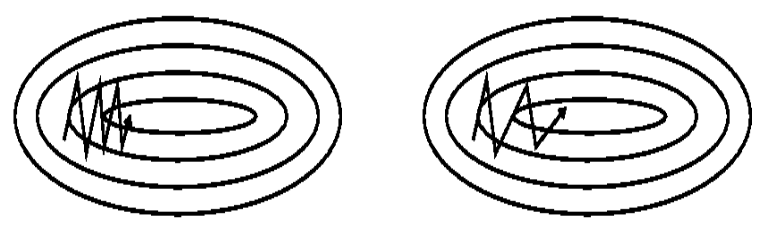
\includegraphics[width = 6in]{../images/momentum}}
\centerline{\Large Rudin's blog}

\vfill
Focusing on the Hessian.

\slide{Quasi-Newton Methods}

It is often faster and more effective to approximate the Hessian.

\vfill
Maintain an approximation $M \approx H^{-1}$.

\vfill
Repeat:

\vfill
\begin{itemize}
\item $\Phi \;\minuseq \; \eta M \nabla_\Phi \;f(\Phi)$ ($\eta$ is often optimized in this step).

\vfill
\item Restimate $M$.
\end{itemize}

\vfill
The restimation of $M$ typically involves a finite difference

\vfill
$$\left(\nabla_\Phi \;f(\Phi)\;|_{\Phi_{t+1}}\right) - \left(\nabla_\Phi \;f(\Phi)\;|_{\Phi_t}\right)$$

\vfill
As a numerical approximation of $H \Delta \Phi$.

\slide{Quasi-Newton Methods}

Conjugate Gradient

\vfill
BFGS

\vfill
Limited Memory BFGS

\slide{Issues with Quasi-Newton Methods}

In SGD the gradients are random even when $\Phi$ does not change.

\vfill
We cannot use

\vfill
$$\left(\nabla_\Phi \;f_{t+1}(\Phi)|_{\Phi_{t+1}}\right) - \left(\nabla_\Phi \;f_t(\Phi)\;|_{\Phi_t}\right)$$

\vfill
as an estimate of $H \Delta \Phi$.

\slide{Issues}

\vfill
\begin{itemize}
\item {\bf Gradient Estimation.} The accuracy of $\hat{g}$ as an estimate of $g$.

  \vfill
\item {\bf Gradient Drift (second order structure).} The fact that $g$ changes as the parameters change.

  \vfill
\item {\bf Convergence.} To converge to a local optimum the learning rate must be gradually reduced toward zero.
\end{itemize}

\slide{The Classical Convergence Theorem}

$$\Phi_{t+1} \;=\; \Phi_t - \eta_t \nabla_\Phi\;\mathrm{loss}(\Phi,x_t,y_t)$$

\vfill
For sufficiently smooth loss functions, {\color{red} and holding the coordinate system constant through time}, and for

$$\eta_t > 0\;\;\;\;\mbox{and}\;\;\;\;\lim_{t \rightarrow \infty} \;\eta_t = 0\;\;\;\;\mbox{and}\;\;\;\;\sum_t \eta_t = \infty,$$

\vfill
the loss value of SGD converges.

\ignore{  This is still wrong.
\slide{More General Convergence Theorem}

$$\Phi_{t+1} \;=\; \Phi_t - \Delta \Phi_t$$

\vfill
$$\tilde{\Delta} f_t \;\doteq\; \left[E_{x_t,y_t} \nabla_\Phi \mathrm{Loss}(\Phi,x_t,y_t)\right]E_{x_t,y_t}\;\Delta \Phi_t(x_t,y_t)$$

$$\mbox{If}\;\;\;\tilde{\Delta}f_t > 0\;\;\;\;\mbox{and}\;\;\;\;\lim_{t \rightarrow \infty} \;\tilde{\Delta}f_t = 0
\;\;\;\;\mbox{and}\;\;\;\;\sum_t \tilde{\Delta}f_t = \infty,$$

\vfill
then the loss value of SGD converges.

\vfill
{\large Warning: I don't know a reference for this.}
}

\slide{Structure From Motion}

\centerline{See the Videos}

https://www.youtube.com/watch?v=i7ierVkXYa8

http://www.mada.org.il/brain/Shape/shape.html

\slide{The Levenberg-Marquart Algorithm (Bundle Adjustment)}

\begin{eqnarray*}
  \mathrm{Loss} & = & E_{(x,y) \sim \mathrm{Train}}\;\frac{1}{2}||f_\Phi(x) - y||^2 \\
  \\
  \\
  f_{\Phi + \Delta \Phi}(x_t) & \approx & f_\Phi(x_t) + J_t\Delta \Phi \\
  \\
  J_t & = & \nabla_\Phi \;f_\Phi(x_t) \\
  \\
  \hat{g}_t & = & (f_\Phi(x_t) - y_t) J_t \;\;= r_tJ_t \\
  \\
  r_t & = & f_\Phi(x_t) - y_t 
\end{eqnarray*}

\slide{The Levenberg-Marquart Algorithm}

\begin{eqnarray*}
    \mathrm{Loss}(\Phi + \Delta \Phi) & \approx & E_t\;\;\frac{1}{2}||r_t + J_t\Delta\Phi||^2
\end{eqnarray*}

\vfill
Minimizing this squared error over the choice of $\Delta \Phi$ is a least squares regression problem.

\begin{eqnarray*}
  0 & = & E_t\; (r_t + J_t \Delta \Phi)J_t \\
  \\
  0 & = & (E_t\;r_tJ_t) + E_t \;J_t^\top J_t \Delta \Phi \\
  \\
  (E_t\; J_t^\top J_t) \Delta \Phi & = & - E_t\; \hat{g}_t \\
  \\
  \Delta \Phi & = & - (E_t\; J_t^\top J_t)^{-1} (E_t\; \hat{g}_t)
\end{eqnarray*}

\slideplain{A General Loss Function}

\begin{eqnarray*}
  \mathrm{Loss}_t(f(\Phi + \Delta \Phi))  & \approx & L_t + \hat{g}_t^\top \Delta \Phi + (J_t\Delta \Phi)^\top H_t\;J_t \Delta \Phi \\
  \\
  J_t & \doteq & \nabla_\Phi \; f(\Phi) \\
  \\
  H_t & \doteq & \nabla_f \nabla_f \; \mathrm{Loss}_t(f)
\end{eqnarray*}

\vfill
Setting the gradient to zero and solving for $\Delta \Phi$:

\begin{eqnarray*}
\Delta \Phi_t & = & - (E_t \;\; J_t^\top H_t\; J_t)^{-1} \hat{g}_t
\end{eqnarray*}


\slide{The Levenberg-Marquart Algorithm for Log Loss}

$$\Phi_{t+1} = \Phi_t - \eta (E_t \;\; J_t^\top H_t\; J_t)^{-1} \hat{g}_t$$

\begin{eqnarray*}
\mathrm{Loss}(\Phi,x,y) & = & -\log Q_{f_\Phi(x)}(y) \\
\\
Q_f(y) & = & \softmax_y f(y) \\
\\
H_t & = & E_{y \sim Q_{f_t}}(\delta_y - Q_{f_t})(\delta_y -Q_{f_t})^\top \\
\\
& = & \mathrm{Diag}(Q_{f_t}) - Q_{f_t}Q_{f_t}^T
\end{eqnarray*}


\slide{END}

} \end{document}
